%----------------------------------------------------------------------------------------
%	Metropolia Thesis LaTeX Template
%----------------------------------------------------------------------------------------
% License:
% This work is licensed under the Creative Commons Attribution 4.0 International License.
% To view a copy of this license, visit http://creativecommons.org/licenses/by/4.0/.
%
% However, this license apply to this template. As a template, it is supposed to be
% modified for your own needs (with your thesis content). For this reason, if you use
% this project as a template and not specifically distribute it as part of a another
% package/program, we grant the extra permission to freely copy and modify these files as
% you see fit and even to delete this copyright notice.
% In short, you are free to publish your thesis under whatever license you wish, even
% keep the all rights reserved to you.
%
% Authors:
% Panu Leppäniemi, Patrik Luoto, Mikaa Oni and Patrick Ausderau
%
% Credits:
% Panu Leppäniemi: abstract, def, cleaning,...
% Patrik Luoto: title page, abstract in Finnish, abbreviation, math,...
% Mikaa Oni: switch to biber biblatex
% Patrick Ausderau: initial version, style, table of content, bibliography, figure,
%                   appendix, table, source code listing,...
%
% Please:
% If you find mistakes, improve this template and alike, please contribute by sharing
% your improvements and/or send us your feedback there:
% https://github.com/panunu/metropolia-thesis-latex
% And of course, if you improve it, add yourself as an author.
%
% Compiler:
% Use XeLaTeX as a compiler. LuaLaTeX works too.
% Typical compilation:
% # minted require -shell-escape to run  external script.
% # -8bit avoid ^^I for tabs in minted.
% $ xelatex -shell-escape -8bit main
% # If any change in the bibliography
% $ biber main
% # If any change with the abbreviation or acronym
% $ makeglossaries main
% #Then compile again
% $ xelatex -shell-escape -8bit main
% #And if still some citation or label warnings, compile once more
% $ xelatex -shell-escape -8bit main

%----------------------------------------------------------------------------------------
%	THESIS INFO
%----------------------------------------------------------------------------------------

% All general information (main language, title, author (you), degree programme, major
% option, etc.)
% Edit the file chapters/0info.tex to change these information
\documentclass[12pt,a4paper,oneside,article]{memoir}%Do not touch this first line ;)

% Global information (title of your thesis, your name, degree programme, major, etc.)

\def\bilingual{yes}%For Finnish students, you must have 2 abstracts, one in English and one in your native language (Finnish or Swedish), so "yes", your thesis is bilingual.
%\def\bilingual{no}%For international student writing in English, only one language and one abstract.

\def\thesislang{finnish} %change this depending on the main language of the thesis.
%\def\thesislang{english} % "english" is the only other supported language currently. If someone has the swedish, please contribute!

\def\secondlang{english} %if the main language is Finnish (or Swedish), you must have 2 abstracts (one in Finnish (or Swedish) and one in English)
%\def\secondlang{finnish}
%If the main language is English and that you are native Finnish (or Swedish) speaker, you must have also abstract in your native language on top of the English one.

\author{Heikki Ketoharju} %your first name and last name

%\def\alaotsikko{Alaotsikko/Subtitle} %DISABLED, seems not to be an option with the 2018 template. If you really need it, uncomment and modify style/title.tex accordingly.

%License
%When publishing your thesis to theseus.fi, you can keep all rights reserved to you,
%or use one of the Creative Commons https://creativecommons.org/licenses/?lang=en
%This attribute will set the license in the metadata of the generated pdf.
%possible options (case sensitive):
%all (keep all rights reserved to yourself)
%by (Attribution)
%by-sa (Attribution-ShareAlike)
%by-nd (Attribution-NoDerivs)
%by-nc (Attribution-NonCommercial)
%by-nc-sa (Attribution-NonCommercial-ShareAlike)
%by-nc-nd (Attribution-NonCommercial-NoDerivs)
%Note that theseus do not accept dedication to public domain CC0
\def\thesiscopy{all}

%Finnish section, for title/abstract
\def\otsikko{Jaettua kieltä etsimässä – GraphQL-rajapinta tietomallin kohentelun
välineenä}
\def\tutkinto{Insinööri (AMK)} % change to your needs, e.g. "YAMK", etc.
\def\kohjelma{Tieto– ja viestintätekniikka}
\def\suuntautumis{Ohjelmistotuotanto}
\def\thesisfi{Insinöörityö}%was Opinnäytetyö
\def\ohjaajat{
Titteli Etunimi Sukunimi\newline
Titteli Etunimi Sukunimi
}
\def\tiivistelma{
Tämä on tiivistelmän ensimmäinen kappale. Tiivistelmän kappaleet loppuvat komentoon newline, jotta saadaan yksi tyhjä rivi aikaiseksi. \newline

Tämä on tiivistlemän toinen kappale.
}
\def\avainsanat{avainsana, avainsana}
\def\aihe{Lyhyt kuvaus opinnäytetyöstä. Max 255 merkkiä.}%for the pdf metadata/properties. If not used, empty it and also the \def\subject.

%English section, for title/abstract
\title{Your title here}
\def\metropoliadegree{Bachelor of Engineering} % change to your needs, e.g. "master", etc.
\def\metropoliadegreeprogramme{your degree programme (e.g. Information Technology)}
\def\metropoliaspecialisation{your major option (e.g. Mobile Solutions)}
\def\thesisen{Bachelor’s Thesis} % change to your need, e.g. master's
\def\metropoliainstructors{
First name Last name, Title (e.g.: Project Manager)\newline
First name Last name, Title (e.g.: Principal Lecturer)
}
\def\abstract{
Abstract content. To force newline between paragraph in the abstract, you must have both a empty line and the newline command. \newline

beginning of second paragraph\ldots
}
\def\metropoliakeywords{keyword, keyword}
\def\subject{short description of the thesis. Max 255 characters.}%for the pdf metadata/properties. If not used, empty it and also the \def\aihe.


%----------------------------------------------------------------------------------------
%	GLOBAL STYLES
%----------------------------------------------------------------------------------------

% If you need extra package, etc. modify the style/style.tex file.
% If you are using Windows OS, you will need to change default font to Arial in that
% style/style.tex file (or install Liberation Sans font to your system).
% If you are using MacOS or linux, make sure you have Liberation Sans font installed.
% Global style. Normally should not be edited.
% If you use windows OS, eventually change \setmainfont to Arial
% Check around commit https://github.com/panunu/metropolia-thesis-latex/commit/a0c15ac77bab1a52c59c517a18080938e57bf5ef
% to see how the font files were manually added (after downloading them: https://pagure.io/liberation-fonts/ )

%\usepackage[l2tabu, orthodox]{nag}%check for obsolete packages (with outdated nag package?)

%condition e.g. for adding or not space in TOC,...
\usepackage{etoolbox}
\ifdefstring{\bilingual}{yes}{
  \usepackage[\secondlang,\thesislang]{babel}% finnish (or swedish) and english
}{
  \usepackage[\thesislang]{babel}% english only
}
\usepackage{iflang}
\usepackage{amsmath}
\usepackage{amsfonts}%extra mathematical symbols
\usepackage{amssymb}
\usepackage{fontspec}
\usepackage{titlesec}
\usepackage{mathtools}%enhance the appearance of documents containing a lot of mathematics
\usepackage[amssymb]{SIunits}
\usepackage[version=3]{mhchem}
\usepackage{tikz} % mindmaps, flowcharts, piecharts, examples at http://www.texample.net/tikz/examples/
\usetikzlibrary{shapes.geometric, arrows}

\usepackage{ragged2e}
\IfLanguageName{finnish}{
  \RaggedRight%2021 template, align left and hyphennization for Finnish version
  \setlength{\RaggedRightRightskip}{0pt plus 1fil}%TODO: fix the Overfull/Underfull warnings when \RaggedRight (likely in title and abstact)
}{}
\makeatletter
  \let\@gnewline\@raggedtwoe@saved@gnewline% Restore original functionality of \newline
  \let\\\@raggedtwoe@savedcr% Restore original functionality of \\
\makeatother

%for compact list
\usepackage{enumitem}
%\usepackage{verbatim}%for block comment
%forcing single line spacing in bibliography
\DisemulatePackage{setspace}
\usepackage{setspace}
%\usepackage{eurosym}%euro symbol
%try to count
\usepackage{totcount}
%insert source code
%require -8bit -shell-escape in the xelatex compile command
%if compiling locally, consider options cachedir=minted,outputdir=~/.tex
\usepackage[newfloat]{minted}
\setminted{tabsize=2,linenos,breaklines,breaksymbolleft={\quad},baselinestretch=1}
\setmintedinline{breaklines,breakanywhere}
\usepackage[singlelinecheck=false]{caption}
%force the width of a table instead of column
\usepackage{tabularx}
\usepackage{booktabs} %why not booktabs? :3

\usepackage{csquotes}% avoid warning with babel

\usepackage{float} % For forced figure location with modifier H (\begin{figure}[H])
\usepackage{wrapfig}

% citep-macro for reference with period inside square brackets [1.]
\newcommand{\citep}[1]{
 \renewcommand\citeright{.]}
 \cite{#1}
 \renewcommand\citeright{]}
}

%set date format to D.M.YYYY
\def\pvm{\the\day.\the\month.\the\year}
%set date format to D Month YYYY
\usepackage[en,useregional=false]{datetime2}
\DTMsetup{datesep=.}
\DTMnewdatestyle{dMonthyyyy}
{%
  \renewcommand{\DTMdisplaydate}[4]{%
    \number##3 % day
    ~% separator
    \DTMenglishmonthname{##2}% month name
    ~% separator
    \number##1% year
  }%
  \renewcommand{\DTMDisplaydate}[4]{%
    \DTMdisplaydate{##4}{##3}{##2}{##1}%
  }%
}
\DTMsetdatestyle{dMonthyyyy}
\date{\today}

\newcommand\tn[1]{\textnormal{#1}} %use \tn instead of \textnormal
\newcommand\reaction[1]{\begin{equation}\ce{#1}\end{equation}} %\reaction{} for chemical reactions

%NORMAL TEXT
%all text, title, etc. in the same font: Arial
%NOTE: fontname is case-sensitive
\setmainfont[Scale=0.98]{Liberation Sans}
%line space
\linespread{1.46}
\AtBeginEnvironment{tabular}{\singlespacing}
%\doublespacing
%margin
%geometry moved after hyperref
\setlength{\parindent}{0pt} %first line of paragraph not indented
\setlength{\parskip}{16.5pt} %one empty line to separate paragraph
%list with small line space separation
\tightlists
\setlist[itemize]{before=\singlespacing,itemsep=6pt,leftmargin=63pt,labelsep=22pt,topsep=1.5pt,partopsep=0pt,after=\vspace{-22pt}\newline}
\setlist[enumerate]{before=\singlespacing,itemsep=6pt,leftmargin=63pt,labelsep=22pt,topsep=1.5pt,partopsep=0pt,after=\vspace{-22pt}\newline}

%IMAGE - FIGURE
%the figures should be placed in the "illustration" folder
\graphicspath{{illustration/}}
%figure number without chapter (1.1, 1.2, 2.1) to (1, 2, 3)
\counterwithout{figure}{chapter}
%border around images
\setlength\fboxsep{0pt}
\setlength\fboxrule{0.5pt}
%space after figure caption (and other float elements)
\setlength{\belowcaptionskip}{-7pt}
\setlength{\intextsep}{16.5pt}%space around floats
\AtBeginEnvironment{table}{\addvspace{16.5pt}}

%TABLE
\counterwithout{table}{chapter}

%SOURCE CODE
\newenvironment{code}{\captionsetup{type=listing}}{}
\IfLanguageName{finnish}{\SetupFloatingEnvironment{listing}{name=Koodiesimerkki}}{}%was Listaus
%\counterwithout{lstlisting}{chapter}
%moved after begin document, otherwise does not compile

%TOC
%change toc title
\IfLanguageName{finnish}{\addto{\captionsfinnish}{\renewcommand*{\contentsname}{Sisällys}}}{}
%remove dots
\renewcommand*{\cftdotsep}{\cftnodots}
%chapter title and page number not in bold
\renewcommand{\cftchapterfont}{\normalfont}
\renewcommand{\cftchapterpagefont}{\normalfont}
%sub section in toc
\setcounter{tocdepth}{2}
%subsection numbered
\setcounter{secnumdepth}{2}
\renewcommand{\tocheadstart}{\vspace*{-33.5pt}}
\renewcommand{\printtoctitle}[1]{\fontsize{13.5pt}{13.5pt}\bfseries #1\vspace*{-4pt}}
%\renewcommand{\aftertoctitle}{\vspace*{-22pt}\afterchaptertitle}
%spacing after a chapter in toc
\preto\section{%
  \ifnum\value{section}=0\addtocontents{toc}{\vskip11pt}\fi
}
%spacing after a section in toc
\renewcommand{\cftsectionaftersnumb}{\vspace*{-3pt}}
%spacing after a subsection in toc
\renewcommand{\cftsubsectionaftersnumb}{\vspace*{-1pt}}
%appendix in toc with "Appendix " + num
\IfLanguageName{finnish}{
  \renewcommand*{\cftappendixname}{Liite\space}
  \renewcommand{\appendixtocname}{Liitteet}
}{\renewcommand*{\cftappendixname}{Appendix\space}}
%appendix header
\IfLanguageName{finnish}{\def\appname{Liite\space}}{\def\appname{Appendix\space}}

%TITLES
%chapter title
%\clearforchapter{\clearpage}
\titleformat{\chapter}
{\fontsize{14pt}{14pt}\bfseries\linespread{1}}%\clearpage
{\thechapter}{.5cm}{}
\titlespacing*{\chapter}{0pt}{21.5pt}{.5pt}
\titleformat{\section}
{\fontsize{13.5pt}{13.5pt}\normalfont}
{\thesection}{.5cm}{}
\titlespacing*{\section}{0pt}{9pt}{0pt}
\titleformat{\subsection}
{\fontsize{12.7pt}{12.7pt}\normalfont}
{\thesubsection}{.5cm}{}
\titlespacing*{\subsection}{0pt}{11pt}{0pt}


%QUOTE
\renewenvironment{quote}
{\list{}{\rightmargin=0pt\leftmargin=2.2cm\topsep=-14pt}%
  \item\relax\singlespacing}%\fontsize{10pt}{10pt}
    {\vspace{8pt}\endlist}

%BIBLIOGRAPHY
%TODO: toggle for Harward v.s. Vancouver
\usepackage[
backend=biber,
bibencoding=utf8,%
citetracker=true,%
isbn=false,%
doi=false,%
url=true,%
usetranslator=true,%
bibstyle=ext-authoryear,%
citestyle=numeric-comp,%
sorting=none,%
sortcites=true,%
block=none,%
terseinits=false,%
giveninits=false,%
maxbibnames=99,%
]{biblatex}

\setlength{\bibitemsep}{11pt}
\setlength{\biblabelsep}{1cm}%with 1cm horizontal gap

\makeatletter
\RequireBibliographyStyle{numeric}
\makeatother

% set right format
\renewcommand*{\multicitedelim}{;\space}
\renewcommand*{\multinamedelim}{;\space}
\renewcommand*{\finalnamedelim}{~\&\space}
\DeclareFieldFormat{biblabeldate}{#1}
\DeclareDelimFormat[bib]{nameyeardelim}{\addperiod\space}
%\DeclareNameAlias{sortname}{last-first} % deprecated
\DeclareNameAlias{default}{family-given}
\DeclareFieldFormat{labelnumberwidth}{#1} % remove () from label number
\DeclareFieldFormat{title}{#1} % normal font for title
\DeclareFieldFormat{citetitle}{#1}
\DeclareFieldFormat{journaltitle}{#1} % remove underline
\DeclareFieldFormat*{url}{%
\ifentrytype{online}{\IfLanguageName{finnish}{Verkkoaineisto}{Online}\addperiod\space}{}%
\ifentrytype{video}{Video\addperiod\space}{}%
\textless\url{#1}\textgreater\addperiod
} % you can modify how to url looks here
%TODO: remove leading 0 for day and month for Finnish dates
\DeclareFieldFormat{urldate}{\space\bibstring{urlseen}\space#1} % remove () from date
%try set translation to biblio
\DefineBibliographyStrings{english}{%
    urlfrom = {available at},%
    urlseen = {Visited on},%
    fromenglish = {from English},%
    fromfinnish = {from Finnish},%
    fromgerman = {from German},%
    fromjapanese = {from Japanese},%
}
\DefineBibliographyStrings{finnish}{%
  %  urlfrom={Linkki: },%
    urlfrom = {},%
    urlseen = {Luettu},%
    fromjapanese = {japanista},%
    fromenglish = {englannista},%
    fromfinnish = {suomesta},%
    fromgerman = {saksasta},%
}
{
  %new cite command: "Vancouver Short"
  \DeclareCiteCommand{\citeVS}
    {\usebibmacro{prenote}}
    {\usebibmacro{author}, \usebibmacro{title}}
    {\multicitedelim}
    {\usebibmacro{postnote}}

  % new cite command: "Vancouver Short Collection" - necessary when referencing whole collections.
  \DeclareCiteCommand{\citeVSc}
    {\usebibmacro{prenote}}
    {\usebibmacro{editor}, \usebibmacro{title}}
    {\multicitedelim}
    {\usebibmacro{postnote}}
}

\addbibresource{biblio.bib}% for biblatex you need out \printbibliography too

%count the appendices (since the chapter counter is reset after \appendix).
%! require to complie 2 times
\regtotcounter{chapter}

% metadata (title, author, lang,...) for accessibility, etc.
\usepackage{hyperref}
\usepackage{hyperxmp}
\def\isolang{\IfLanguageName{finnish}{fi}{en}} %iso code (based on main language)
\ifdefstring{\thesiscopy}{all}{%
    \def\copyen{Copyright \textcopyright\ \the\year{}, \theauthor}
    \def\copyfi{Kaikki oikeudet pidätetään.  \textcopyright\ \the\year{}, \theauthor}
  }{%
    \usepackage[type={CC},modifier={\thesiscopy},version={4.0},]{doclicense}
    \def\copyen{\thetitle\ \textcopyright\ \the\year{} by \theauthor\ is licensed under \doclicenseLongNameRef}
    \def\copyfi{\otsikko\ \textcopyright\ \the\year{}, jonka tekijä on \theauthor, on lisensoitu \doclicenseLongNameRef}
}
\hypersetup{%
  pdfdisplaydoctitle,
  %breaklinks=true,%searching for overfull warnings
  pdfencoding=auto,
  bookmarksdepth=subsection,
  unicode=true,
  keeppdfinfo=true,
  pdflang={\isolang},
  pdfmetalang={\isolang},
  pdftitle={\IfLanguageName{finnish}{\otsikko}{\thetitle}},
  pdfkeywords={\IfLanguageName{finnish}{\avainsanat}{\metropoliakeywords}},
  pdfcopyright={\IfLanguageName{finnish}{\copyfi}{\copyen}},
  pdfsubject={\IfLanguageName{finnish}{\aihe}{\subject}},
}

\ifdefstring{\bilingual}{yes}{%metadata (title and copyright) in multiple language
  \XMPLangAlt{\IfLanguageName{finnish}{en}{fi}}{%
    pdftitle={\IfLanguageName{finnish}{\thetitle}{\otsikko}},
    pdfcopyright={\IfLanguageName{finnish}{\copyen}{\copyfi}},
    pdfsubject={\IfLanguageName{finnish}{\subject}{\aihe}},
  }
}{}
\urlstyle{same}

%moved after hyperred as can cause conflicts
\usepackage{pdfcomment}%try the alt text for graphics
\usepackage{accsupp}
\newcommand{\AltText}[2]{\BeginAccSupp{method=pdfstringdef,unicode,Alt={{#1}}}\pdftooltip{{#2}}{{#1}}\EndAccSupp{}}

\usepackage[top=2.5cm, bottom=3cm, left=4cm, right=2cm, nofoot]{geometry}

\usepackage{pgfplots} %simple plots etc
\pgfplotsset{compat=1.16}
\usepackage{pgfplotstable}

% Abbreviations, acronym and glossary, in case of bug, remove temporary the noredefwarn
\usepackage[acronym,toc,nonumberlist,section=chapter,noredefwarn]{glossaries}%xindy,%toc, ,nomain
\newglossarystyle{mystyle}{%
  \setglossarystyle{list}% base this style on the list style
  \renewcommand*{\glossentry}[2]{%
  \item[\glsentryitem{##1}%
    \glstarget{##1}{\glossentryname{##1}:}]
  \glossentrydesc{##1}\glspostdescription\space ##2}
}
\setglossarystyle{mystyle}

\renewcommand*{\glsclearpage}{}

% Normally, you do not need to modify the title style. It's content comes from the
% chapters/0info.tex file.
\input{style/title.tex}

%----------------------------------------------------------------------------------------
%	ABBREVIATION AND GLOSSARY
%----------------------------------------------------------------------------------------

% Add/edit all your acronyms, abbreviations, glossary entries, etc. definitions in
% chapters/0abbr.tex file.
% You can have as many as you wish. Only the ones you use in your text (inserted with
% \gls{} command) will print in the Glossary/Lyhenteet.
% Generate the glossary
\makeglossaries

% Acronyms, abbreviations, etc.

\newacronym{lamp}{LAMP}{LAMP (Linux, Apache, MySQL, PHP)}
\newacronym{orm}{ORM}{Object-relational mapper, oliot tietokantatauluiksi muuntava teknologia}
\newacronym{sql}{SQL}{Structured Query Language}
\newacronym{io}{I/O}{Input/Output}
\newacronym{ram}{RAM}{Random Access Memory}
\newacronym{php}{PHP}{Hypertext Preprocessor}
\newacronym{wysiwym}{WYSIWYM}{What You See Is What You Mean}
\newacronym{isbn}{ISBN}{International Standard Book Number}
\newacronym{url}{URL}{Uniform Resource Locator}
\newacronym{doi}{DOI}{Digital Object Identifier}


\newacronym{html}{HTML}{HyperText Markup Language}


% Glossary entries
\newglossaryentry{ddd}{
  name={Sovellusaluevetoinen suunnittelu},
  text={sovellusaluevetoinen suunnittelu},
  description={Menetelmä, jossa ohjelmistoa kehitetään läheisessä yhteistyössä sovellusalueen asiantuntijoiden kanssa. (myös: Liiketoimintavetoinen suunnittelu.) Engl. Domain Driven Design}
  }
\newglossaryentry{domain}{
  name={Sovellusalue},
  text={sovellusalue},
  description={Erityisala, jota sovellus käsittelee. Esimerkiksi pankkitoiminta tai vähittäiskauppa. myös: liiketoimintataso}
}

\newglossaryentry{crunching}{
  name={Tiedon rouhinta},
  text={tiedon rouhinta},
  description={Prosessi, jossa tunnistetaan sovellusalan erityiskäsitteitä ohjelmoijan ja sovellusalueen asiantuntijan välisen kommunikaation avulla. Engl. Knowledge crunghing}
  }
\newglossaryentry{dsl}{
  name={Täsmäkieli},
  text={täsmäkieli},
  description={Erityisalaan liittyvä formaali kieli. Esimerkiksi ohjelmointi- tai kuvauskieli. Engl. Domain-Specific language}
  }
\newglossaryentry{ubilang}{
  name={Kaikenkattava kieli},
  text={kaikenkattava kieli},
  description={Kokoelma käsitteitä ja sanastoa, joiden avulla ohjelmoijat ja sovellusalueen asiantuntijat keskustelevat kehitettävästä ohjelmistosta. Muotoutuu tiedon rouhintaprosessin tuloksena. Engl. Ubiquitous language}
  }
\newglossaryentry{domainmodel}{
  name={Sovellusaluemalli},
  text={sovellusaluemalli},
  description={Käsitteistä ja niiden välisistä suhteista koostuva, ohjelmakoodin muotoon kaapattava malli käsiteltävästä sovellusalueesta. Engl. Domain Model}
  }
\newglossaryentry{domainlayer}{
	name={Liiketoimintalogiikan taso},
	text={liiketoimintalogiikan taso},
	description={Ohjelmiston sisäinen osa, joka pitää sisällään liiketoimintaan liittyvän ohjelmalogiikan. Engl. Domain layer},
}
\newglossaryentry{entity}{
	name={Yksilötyyppi},
	text={yksilötyyppi},
	description={Ohjelmassa esiintyvä olio, jolla on identiteetti. Esimerkiksi yksittäinen asiakas tai lasku. Engl. Entity},
}
\newglossaryentry{deepermodel}{
  name={Syvempi malli},
  text={syvempi malli},
  description={Sovellusaluevetoisen suunnittelun myötä parantunut sovellusaluemalli. Syvempi malli tavoittaa aiempaa paremmin sovellusalan perimmäisen luonteen. Engl. Deeper Model}
}
\newglossaryentry{hakurakenne}{
  name={Assosiaatiotaulu},
  text={assosiaatiotaulu},
  description={Engl. Map. suom. myös {\em hakurakenne\/} ja {\em sanakirja\/}. Tietorakenne, joka sisältää joukon avain-arvo -pareja}
}

\newglossaryentry{rest}{
  name={REST},
  text={REST},
  description={Representational State Transfer. Arkkitehtoninen tyyli rajapintojen määrittelemiseen etenkin Web-sovelluksissa}
}

\newglossaryentry{graphql}{
  name={GraphQL},
  text={GraphQL},
  description={Facebookin kirjoittama kyselykieli, joka esittää manipuloitavan datan olioverkkona}
}

\newglossaryentry{http}{
  name={HTTP},
  text={HTTP},
  description={Hypertext Transfer Protocol. Webin perusprotokolla, jota käytetään hypertekstidokumenttien siirtoon}
}

\newglossaryentry{verkko}{
  name={Verkko},
  text={verkko},
  description={Tietorakenne, joka koostuu solmuista ja kaarista}
}

\newglossaryentry{domainexpert}{
  name={Alan asiantuntija},
  text={alan asiantuntija},
  description={Sovellusalueen esimerkiksi työnsä puolesta hyvin tunteva henkilö}
}

\newglossaryentry{kulkusuunta}{
  name={Kulkusuunta},
  text={kulkusuunta},
  description={Olioita yhdistävän kytköksen suunta}
}

\newglossaryentry{puhdasfunktio}{
  name={Puhdas funktio},
  text={puhdas funktio},
  description={Funktio, jonka palauttama tulos riippuu vain sen saamien parametrien arvoista. Puhdas funktio ei aiheuta sivuvaikutuksia esimerkiksi tulostamalla ruudulle tai tallentamalla tiedostoon}
}

\newglossaryentry{tyyppi}{
  name={Tyyppi},
  text={tyyppi},
  description={Lausekkeeseen sidottu määritys lausekkeen palauttaman arvon tietotyypistä. Esimerkiksi kokonaisluku tai merkkijono}
}

\newglossaryentry{aggregate}{
  name=Aggregaatti,
  text=aggregaatti,
  description={Useiden olioiden kokoelma, jolla on yksi juuriolio. Käsitellään ohjelmalogiikassa yhtenä kokonaisuutena.}
}
\newglossaryentry{repository}{
  name=Repositorio,
  text=repositorio,
  description=Rajapinta tiedon tallennusvälineeseen
}
\newglossaryentry{factory}{
  name=Tehdas-olio,
  text=tehdas-olio,
  description={Olio, joka vastaa toisten olioiden luomisesta}
}



%----------------------------------------------------------------------------------------
%	DOCUMENT STARTS HERE...
%----------------------------------------------------------------------------------------

\begin{document}
\IfLanguageName{finnish}{
}{
  \raggedright%2021 template, align left, no hyphennization for English version
}
\counterwithout{listing}{chapter}

%----------------------------------------------------------------------------------------
%	TITLE PAGE
%----------------------------------------------------------------------------------------

\input{style/title_headers.tex}
\maketitle
\newpage

%----------------------------------------------------------------------------------------
%	ABSTRACT / Tiivistelmä
%----------------------------------------------------------------------------------------

% If you are international student writing in English, ignore the Finnish abstract.
% If you are Finnish citizen, you must have 2 abstracts, one in Finnish (or Swedish
% depending on your mother tongue) and one in English regardless of the main language of
% your thesis. Normally, you do not need to modify the abstract style. It's content comes
% from the chapters/0info.tex file.
\ifdefstring{\bilingual}{no}{%
    \input{style/abstract_en.tex}
    }{%
    \IfLanguageName{finnish}{%order of abstracts based on main language and spacing hell
        % Abstract in Finnish
% Normally, you should not edit this file. Everything comes from chapter/0info.tex

\pagestyle{empty} %remove page number
\newgeometry{top=1.5cm,left=4cm,right=.5cm}
\begin{otherlanguage}{finnish}
{\large\textbf{Tiivistelmä}}
{\renewcommand{\arraystretch}{1.1}
  \begin{tabular}{@{}p{4.7cm} >{\raggedright\arraybackslash}p{10.8cm}@{}}
  Tekijä: & \makeatletter\@author\makeatother
  \\
  Otsikko: & \otsikko
  \\
  Sivumäärä: & \pageref*{LastPage} sivua
  \\
  Aika: & \pvm
  \\[6.5mm]
  Tutkinto: & \tutkinto
  \\
  Tutkinto-ohjelma: & \kohjelma
  \\
  Ammatillinen pääaine: & \suuntautumis
  \\
  Ohjaajat: & \ohjaajat
  \\[11mm]
  \cmidrule[.7pt](l{-.15em}r{5.5em}){1-2}
  \multicolumn{2}{>{\raggedright}p{15.5cm}}{
  \vspace{.2mm}
  \tiivistelma
  }
  \\
  \\
  Avainsanat: & \avainsanat
  \\
\end{tabular}
}
\end{otherlanguage}
\restoregeometry
\clearpage


        % Abstract in English
% Normally, you should not edit this file. Everything comes from chapter/0info.tex

\pagestyle{empty} %remove page number
\newgeometry{top=1.77cm,left=4cm,right=.5cm}
\begin{otherlanguage}{english}
{\large\textbf{Abstract}}
{\renewcommand{\arraystretch}{1.1}
  \begin{tabular}{@{}p{4.7cm} >{\raggedright\arraybackslash}p{10.8cm}@{}}
  Author: & \makeatletter\@author\makeatother
  \\
  Title: & \makeatletter\@title\makeatother
  \\
  Number of Pages: & \pageref*{LastPage} pages
  \\
  Date: & \makeatletter\thedate\makeatother
  \\[6.5mm]
  Degree: & \metropoliadegree
  \\
  Degree Programme: & \metropoliadegreeprogramme
  \\
  Professional Major: & \metropoliaspecialisation
  \\
  Supervisors: & \metropoliainstructors
  \\[9mm]
  \cmidrule[.7pt](l{-.15em}r{5.5em}){1-2}
  \\
  \multicolumn{2}{>{\raggedright}p{15.5cm}}{
    \abstract
  }
  \\
  \\
  Keywords: & \metropoliakeywords
  \\
\end{tabular}
}
\end{otherlanguage}
\restoregeometry
\clearpage


        }{
        \input{style/abstract_en.tex}
        % Abstract in Finnish
% Normally, you should not edit this file. Everything comes from chapter/0info.tex

\pagestyle{empty} %remove page number
\newgeometry{top=2.04cm,left=4cm,right=.5cm}
\begin{otherlanguage}{finnish}
{\large\textbf{Tiivistelmä}}
{\renewcommand{\arraystretch}{1.1}
  \begin{tabular}{@{}p{4.7cm} >{\raggedright\arraybackslash}p{10.8cm}@{}}
  Tekijä: & \makeatletter\@author\makeatother
  \\
  Otsikko: & \otsikko
  \\
  Sivumäärä: & \pageref*{LastPage} sivua
  \\
  Aika: & \pvm
  \\[6.5mm]
  Tutkinto: & \tutkinto
  \\
  Tutkinto-ohjelma: & \kohjelma
  \\
  Ammatillinen pääaine: & \suuntautumis
  \\
  Ohjaajat: & \ohjaajat
  \\[4mm]
  \cmidrule[.7pt](l{-.15em}r{5.5em}){1-2}
  \\
  \multicolumn{2}{>{\raggedright}p{15.5cm}}{
  \tiivistelma
  }
  \\
  \\
  Avainsanat: & \avainsanat
  \\
\end{tabular}
}
\end{otherlanguage}
\restoregeometry
\clearpage


    }
}
%----------------------------------------------------------------------------------------
%	License? Acknowledgement?
%----------------------------------------------------------------------------------------

% Uncomment next line and edit chapters/0license.tex if you want license in your thesis.
%% License of your thesis
% If you wish to explain what it means. When you publish your thesis in https://theseus.fi
% you will be able to choose between some Creative Commons licenses
% https://creativecommons.org
% Adapt this example text to your taste.
% This would also be the right place to explain the license you choose for the code you
% produced for your thesis.

\pagestyle{empty}
\chapter*{Licenses}
\ifdefstring{\thesiscopy}{all}{}{%
  \begin{wrapfigure}{r}{0.3\textwidth}
    \vspace{-20pt}
    \doclicenseImage
  \end{wrapfigure}
 }
\IfLanguageName{finnish}{\copyfi}{\copyen}

That means:

%adapt to the license you choose. In this example: https://creativecommons.org/licenses/by-sa/4.0/deed.en
\textbf{You are free to:}
\begin{itemize}
\item Share \textemdash copy and redistribute the material in any medium or format
\item Adapt \textemdash remix, transform, and build upon the material
\end{itemize}

\textbf{Under the following terms:}
\begin{itemize}
\item \ccAttribution~ Attribution \textemdash You must give appropriate credit, provide a link to the license, and indicate if changes were made. You may do so in any reasonable manner, but not in any way that suggests the licensor endorses you or your use.
\item \ccShareAlike~ ShareAlike \textemdash If you remix, transform, or build upon the material, you must distribute your contributions under the same license as the original.
\item No additional restrictions \textemdash You may not apply legal terms or technological measures that legally restrict others from doing anything the license permits.
\item Any of the above conditions can be waived if you get my permission
\end{itemize}

%Eventually consider few words why you choose such license? E.g. something like:

Työmallista laatimani havainnekuva käyttää kahta vektorimuotoista kuvaa, joiden
tekijä tulee mainita.
Sivustolta Vecteezy
Doctor and surgeon wearing medical masks käyttäjältä jemastock
Female Developer Vector käyttäjältä biggorilla 298

\clearpage


% Uncomment next line and edit chapters/0acknowledgement.tex if you want acknowledgements.
%\input{chapters/0acknowledgement.tex}

%----------------------------------------------------------------------------------------
%	TABLE OF CONTENTS
%----------------------------------------------------------------------------------------

\input{style/toc.tex}

%list of figure, tables would come here if relevant?

%----------------------------------------------------------------------------------------
%	Lyhenteet / Abbreviation
%----------------------------------------------------------------------------------------

% If you don't use abbreviations/glossary, remove the following line.
% Abbreviation and Glossary
% Normally, you don't have to modify this file. Your abbreviations, etc. goes in
% ../chapters/0abbr.tex file.

\begin{singlespacing}

	% \gsladdall%would add all terms even if not used in your text.
	\addtocontents{toc}{\cftpagenumbersoff{chapter}}
	{
		\vspace{-.46cm}
		\titleformat{\section}
		{\fontsize{13.5pt}{13.5pt}\bfseries\normalfont}
		{\thesection}{.5cm}{}
		\renewcommand*{\glossarypreamble}{\vspace{.7\baselineskip}}
		%Adapt labelwidth (sorry for the ugly hack)
		\setlist[description]{leftmargin=!, labelwidth=4em, before=\doublespacing}
		\IfLanguageName {finnish} {
			\printacronyms[title=Lyhenteet, nogroupskip]
			}{
			\printacronyms[title=List of Abbreviations, nogroupskip]
		}
		\setlist[description]{leftmargin=!, labelwidth=10em}
		\vspace{1cm}
		\printglossary[]
		\setlist[description]{style=standard} % reset settings back to default
	}
	\addtocontents{toc}{\cftpagenumberson{chapter}}
\end{singlespacing}

\clearpage


%----------------------------------------------------------------------------------------
%	CONTENT
%----------------------------------------------------------------------------------------

\input{style/content.tex}%reset page number to 1, etc.

% Thesis content if you strictly follow the "Final Year Project guide". Of course, you
% can adapt to your specific needs (add more chapter, rename them, etc.).
% Introduction

\chapter{Johdanto}

Pitkäikäinen, jatkuvasti kehitetty ohjelma mutkistuu herkästi. Jos kehitystiimi
ei pidä varaansa, alun perin yksinkertaisesta ja selkeästä ohjelmakoodista ja suoraviivaisesta tietorakenteesta kasvaa hankalasti hallittava kokonaisuus.

Sotkuiseenkin ohjelmistoon voi kuitenkin saada selvyyttä taitavalla kohentelulla
ja kehittämisellä. Kun toimintoja alkaa jakaa osiin, ja rakentaa osien välille
selkeitä nivelkohtia, avautuu mahdollisuus tehdä hedelmällisiä parannuksia.

Web-sovelluksessa eräs merkittävimpiä nivelkohtia on sovelluksen käyttöliittymän
ja logiikkaosan välinen HTTP-rajapinta. Tässä insinöörityössä tarkastellaan,
voiko tämän rajapinnan uudistamisen kanssa yhtä aikaa myös kohentaa ohjelmiston sisäistä logiikkaa.

Työ tehdään ohjelmistopalveluyritys Nordhealth Oy:n tilauksesta.
 
\section{Nordhealth Oy lyhyesti}


Nordhealth Oy on vuonna 2001 perustettu ohjelmistopalveluyritys, joka tekee toiminnanohjausjärjestelmiä kahdelle eri toimialalle: Provet Cloud -järjestelmää eläinlääkäriklinikoille ja Diarium-järjestelmää terapeuteille. Molemmat järjestelmät ovat web-pohjaisia sovelluksia. Niitä käytetään kirjautumalla web-selaimen kautta. (Tästä puuttuu perustietoja, kuten työntekijöiden määrä, liikevaihto tms.)

Nordhealthia voisi luonnehtia tyypilliseksi ohjelmistoalan yritykseksi: se tekee
erityisalalle suunnattua toiminnanohjausjärjestelmää. Alunperin järjestelmät
ovat olleet työpöytäsovelluksia, ja siitä Nordhealth on muuntanut ne
LAMP-alustalla toimiviksi web-sovelluksiksi. Kun Web on kehittynyt, on otettu
suunnaksi sovellusten siirtäminen julkiseen pilveen, ja käyttöliittymän
rakentaminen erilliseksi yhden sivun JavaScript-sovellukseksi.

Diarium on Nordhealthin kahdesta järjestelmästä vanhempi. Se on suunnattu terapeuteille: fysio-, toiminta-, puhe- ja psykoterapeuteille. Järjestelmä on laajentunut yksinkertaisesta potilaskortistojärjestelmästä suurenkin terapia-alan yrityksen tarpeita vastaavaksi toiminnanohjausjärjestelmäksi, ja se on lisäksi myös Valviran tarkoittama A-luokan potilastietojärjestelmä. Diariumia käyttävä terapeutti voi siis lähettää käyntikirjaukset potilastiedon sähköiseen Kanta-rekisteriin.

\section{Insinöörityön tavoite}

Työn tavoitteena on analysoida pientä osaa Diariumin tietomallista, ja etsiä
parempia tapoja sen toteuttamiseen. Diariumin HTTP-rajapintaa halutaan muista
syistä kehittää, ja tämä tarjoaa työni pääkysymyksen: onko ohjelmiston
tietomallia mahdollista kehittää rakentamalla GraphQL-rajapinta?

GraphQL on teknologiana uusi ja erilainen verrattuna vanhaan HTTP REST
-rajapintaan. Tarvitaan siis hyviä perusteita siihen siirtymiselle.

Taustateoksena työssä käytän Eric Evansin kirjaa Doman Driven Design.

Työn tuloksena en ajattele syntyvän valmista ja parempaa tietomallia, vaan
pikemminkin prosessi tietomallin kehittämiseksi rajapinnan uusimisen ohella.
% uncomment what you need.
\hypertarget{luxe4htuxf6kohdat-ja-tavoitteet}{%
\chapter{Lähtökohdat ja
tavoitteet}\label{luxe4htuxf6kohdat-ja-tavoitteet}}

\hypertarget{nordhealth-oy-lyhyesti}{%
\section{Nordhealth Oy lyhyesti}\label{nordhealth-oy-lyhyesti}}

Nordhealth Oy on vuonna 2001 perustettu ohjelmistopalveluyritys, joka
tekee toiminnanohjausjärjestelmiä kahdelle eri toimialalle: Provet Cloud
-järjestelmää eläinlääkäriklinikoille ja Diarium-järjestelmää
terapeuteille. Molemmat järjestelmät ovat web-pohjaisia sovelluksia.
Niitä käytetään kirjautumalla web-selaimen kautta. \textbf{(Tästä
puuttuu perustietoja, kuten työntekijöiden määrä, liikevaihto tms.)}

Nordhealthia voisi luonnehtia tyypilliseksi ohjelmistoalan yritykseksi:
se tekee erityisalalle suunnattua toiminnanohjausjärjestelmää.
Tyypillinen on myös järjestelmien kehityskaari: alunperin ne ovat olleet
työpöytäsovelluksia, ja siitä Nordhealth on muuntanut ne LAMP-alustalla
toimiviksi web-sovelluksiksi. Kun Web on kehittynyt, on otettu suunnaksi
sovellusten siirtäminen julkiseen pilveen, ja käyttöliittymän
rakentaminen erilliseksi yhden sivun JavaScript-sovellukseksi.

Diarium on Nordhealthin kahdesta järjestelmästä vanhempi. Se on
suunnattu terapeuteille: fysio-, toiminta-, puhe- ja psykoterapeuteille.
Järjestelmä on laajentunut yksinkertaisesta
potilaskortistojärjestelmästä suurenkin terapia-alan yrityksen tarpeita
vastaavaksi toiminnanohjausjärjestelmäksi, ja se on lisäksi myös
Valviran tarkoittama A-luokan potilastietojärjestelmä. Diariumia
käyttävä terapeutti voi siis lähettää käyntikirjaukset potilastiedon
sähköiseen Kanta-rekisteriin.

\hypertarget{insinuxf6uxf6rityuxf6n-tavoite}{%
\section{Insinöörityön tavoite}\label{insinuxf6uxf6rityuxf6n-tavoite}}

Työn tavoitteena on selvittää, onko ohjelmiston tietomallia mahdollista
parannella rakentamalla GraphQL-rajapinta.

Lisäksi työn myötä on tavoitteena löytää parempi tietomalli osaan
Diarium-sovellusta.

Kolmas tärkeä tavoite on kehittää työmenetelmä, jonka avulla tietomallia
on mahdollista korjata.

Projektin edetessä rakennan pienen GraphQL-rajapinnan ja sitä
hyödyntävän prototyyppisovelluksen. Tämä toimii kokeilukenttänä, jonka
kautta työmenetelmää ja tietomallia etsitään.

\vspace{21.5pt}

\hypertarget{teoria}{%
\chapter{Teoria}\label{teoria}}

Keskeisten käsitteiden esittely

\hypertarget{domain-driven-design}{%
\section{Domain Driven Design}\label{domain-driven-design}}

(Sovellusalakeskeinen suunnittelu) (Liiketoimintavetoinen suunnittelu)

\hypertarget{knowledge-crunching}{%
\subsection{Knowledge crunching}\label{knowledge-crunching}}

\hypertarget{ubiquitous-language}{%
\subsection{Ubiquitous Language}\label{ubiquitous-language}}

\hypertarget{mallin-ilmaiseminen-ohjelmistossa}{%
\subsection{Mallin ilmaiseminen
ohjelmistossa}\label{mallin-ilmaiseminen-ohjelmistossa}}

\begin{itemize}
\tightlist
\item
  Domain-malli on ohjelmistossa omana erillisenä kerroksenaan, puhtaasti
  ja erillään muista.
\item
  Entity - entiteetti, eli olio, jolla on identiteetti
\item
  Assosiaatio, eli kulkusuunta
\end{itemize}

Pohdintaa: - Evans suosittaa kerroksittaista arkkitehtuuria, ja
erillistä kerrosta, jossa Domain-malli elää. Luonteva paikka tälle voisi
olla GraphQL-rajapinnan takana.

\hypertarget{graphql}{%
\section{GraphQL}\label{graphql}}

\hypertarget{tyyppijuxe4rjestelmuxe4}{%
\subsection{Tyyppijärjestelmä}\label{tyyppijuxe4rjestelmuxe4}}

GraphQL-rajapinta koostuu tyypeistä

\hypertarget{query-ja-mutation}{%
\subsection{Query ja Mutation}\label{query-ja-mutation}}

Rajapintaan voi tehdä queryjä - nämä ovat ikäänkuin sisäänmenoaukkoja,
joiden kautta oliorakenteita voi pyytää Mutation - toiminto datan
muuntelemiseen. Myös tämä palauttaa dataa

\hypertarget{skeema}{%
\subsection{Skeema}\label{skeema}}

Rajapinnan tyypit, niille tehtävät kyselyt ja mutaatiot kuvataan
skeemassa, GraphQL-kielen avulla.

-Pohdintaa: Tämä skeema on varmaankin keskeinen nivelkohta Domain Driven
Designin kanssa.

\vspace{21.5pt}

\hypertarget{tyuxf6n-kulku}{%
\chapter{Työn kulku}\label{tyuxf6n-kulku}}

Päätin tehdä työn lyhyissä iteraatioissa, ketterän kehityksen
periaatteita seuraten. Tämä tyyli soveltuu hyvin yhteen tietomallin
kehittämisen kanssa, sillä Evansin kirjassa kuvattu työtapa on
samankaltainen. Lyhyet iteraatiot ovat nykyään tyypillinen tapa tehdä
ohjelmistoa. {[}kenen mukaan?{]}

En asettanut iteraatioille mitään ennalta määrättyä kestoa.

Päätin, että jokainen iteraatio aloitetaan minun ja tuoteomistaja Lauran
välisellä suunnittelukokouksella, jonka pääasiallisena tavoitteena oli
keskustellen ja piirtäen etsiä toimivaa ohjelmiston tietomallia.
Prosessin kuluessa tavaksi vakiintui, että kokouksen aluksi käytiin
nopeasti läpi siihen asti aikaansaadun ohjelmistoprototyypin
toiminnallisuus.

Pyrin noudattamaan työskentelyssä Eric Evansin esittämää tiedon
rouhimisen periaatetta, jossa suunnittelu ja ohjelmistokehitys
limittyvät keskenään.

Iteraation aikana ohjelmoin uuden version ohjelmistoprototyypistä,
kokouksessa syntyneiden ajatusten pohjalta.

\hypertarget{aiheen-valitseminen}{%
\section{Aiheen valitseminen}\label{aiheen-valitseminen}}

Yrityksessä haluttiin valita laskutuksen sisältä tapaus, jossa
hoitokäynti tulee voida jakaa usealle eri maksajalle osoitetuille
laskuille, ja nämä laskut tulee voida hyvittää itsenäisesti.

Mallintamisen aiheeksi valittu laskutus oli aihealueena minulle
tuntematon, ja yksi prosessin haasteita olikin, pystynkö muutamassa
viikossa omaksumaan riittävästi laskutuksen käsitteitä toimivan mallin
aikaansaamiseksi.

\hypertarget{laskutuksen-taustaa}{%
\section{Laskutuksen taustaa}\label{laskutuksen-taustaa}}

Ohjelmistoa käyttävä terapeutti kirjaa järjestelmään hoitokäyntejä ja
laskuttaa niitä. Monesti samalle maksajalle - etenkin, jos tämä ei ole
yksityishenkilö vaan instituutio - kertyy monta eri laskua, jotka
lähetetään yhtenä joukkona esimerkiksi kerran kuukaudessa. Tätä
kutsutaan koontilaskuksi.

Toisinaan jo luodussa laskussa huomataan virhe. Kirjanpidon
periaatteiden mukaan laskuja ei kuitenkaan saa tuhota, vaan virheellinen
lasku on oikaistava tai kumottava. Tässä ohjelmistoprototyypissä
oletetaan, että kyse on aina virheellisesti laskutetusta käynnistä, jota
maksaja kieltäytyy maksamasta, ja joka pitää kumota. Tämä tapahtuu
luomalla hyvityslasku.

Hyvityslasku on voitava luoda siten, että yksittäisellä laskulla oleva
yksittäinen rivi voidaan kumota, muun laskun (ja sen sisältävän
koontilaskun) säilyessä avoimena.

\hypertarget{iteraatio-1}{%
\section{Iteraatio 1}\label{iteraatio-1}}

Iteraation aloittavassa kokouksessa suunnittelimme yksinkertaisen
mallin, jossa hoitokäynnit liittyvät laskuihin, laskut kootaan
koontilaskuille ja koontilaskut hyvityslaskuille.

Tämän mallin sisältävän ohjelmistoprototyypin toteuttamiseen kului kaksi
viikkoa, ja näin iteraatio oli pisin. Kulunutta aikaa selittää, että
rakensin prototyypin puhtaalta pöydältä, jolloin aikaa kului myös
sovelluksen pohjan pystyttämiseen.

Ariadne-GraphQL -kirjastoon ja Falcon-HTTP-kirjastoon piti tutustua,
samoin kuin Pytest-yksikkötestausjärjestelmään.

\hypertarget{iteraatio-2}{%
\section{Iteraatio 2}\label{iteraatio-2}}

Iteraation aloittavassa kokouksessa kävimme läpi syntyneen
ohjelmistoprototyypin. Minua oli koko viikon ajan vaivannut käyntien ja
laskujen läheinen kytkös.

Pyysin Lauraa kertomaan enemmän siitä, mitä käynnin laskuttaminen
oikeastaan tarkoittaa, ja hän piti lyhyen yhteenvedon laskuttamisen
periaatteista. Huomioni kiinnittyi puheessa esiintyneeseen termiin
\textbf{Laskutusperuste}. Tämä tuntui valtavan kiinnostavalta, ja
lähdimme tarkastelemaan sitä eri puolilta.

Tapaamisen jälkeisen viikon kehitystyötä ohjasi nyt uusi ajattelutapa:
käyntiä sinänsä ei liitetä laskuun, vaan käynti laskutetaan, mikäli
laskutusperuste täyttyy.

Toisen tapaamisen aikana syntynyt malli on esitetty kuvassa X. Siinä
jokaiseen käyntiin voidaan liittää palvelurivi, ja palveluriviin
puolestaan hyvitysrivi. Palvelurivi on se, joka lisätään laskulle
käynnin sijasta. Kun halutaan tietää, täyttyykö laskutusperuste, voidaan
tarkastaa, liittyykö käyntiin palvelurivi.

Mallin toteuttamisessa kesti vajaat neljä päivää, ja sain sen toimimaan
perjantaina iltapäivällä. Kokemus oli mielenkiintoinen.

Jotta uusia ominaisuuksia pääsi toteuttamaan, täytyi olemassaolevaa
ohjelmaa aluksi refaktoroida voimakkaasti. Aiemmin suoraan laskulle
kytkettyyn käyntiin piti sijoittaa sisälle palveluriviä kuvaava olio, ja
lasku muuttaa koostumaan näistä. Käynnin ja hyvityslaskun välinen kytkös
piti katkaista, ja tilalle rakentaa kytkös laskurivin ja hyvitysrivin
välille.

Perjantaihin tultaessa olin refaktoroinut prototyyppiohjelmaa ja sen
jälkeen käyttänyt kolme päivää ensimmäisen käyttäjätarinan parissa.
Yllättäen perjantaina puolen päivän jälkeen kaikki yksikkötestit menivät
läpi, tarina valmistui, ja ohjelmistoprototyyppi tuntui toimivan kuin
ajatus. Loppujen kahden käyttäjätarinan toteuttaminen onnistui kahdessa
tunnissa.

Toinen iteraatio kesti yhden viikon.

\hypertarget{iteraatio-3}{%
\section{Iteraatio 3}\label{iteraatio-3}}

Kolmannen iteraation aluksi pidimme jälleen suunnittelukokouksen. Tämän
kokouksen keskeisimpänä ongelmana oli, miten jo kertaalleen laskutettu
ja hyvitetty käynti voidaan laskuttaa uudelleen.

Yritimme piirtää monenlaisia erilaisia malleja ja diagrammeja, mutta
mikään niistä ei tuntunut osuvalta.

Kokouksen lopuksi päätimme, että on hyödyllistä luoda yhdessä joukko
käyttäjätarinoita, joiden pohjalta kehitystä voidaan tehdä. Emme
määritelleet tarinoita tiukan muodollisesti, vaan ainoastaan lauseella
tai kahdella.

Kokouksen jälkeen jouduin tekemään samankaltaisen laajan refaktoroinnin
kuin edellisellä viikolla. Se ei kuitenkaan kestänyt yhtä kauaa.

Ohjelmoidessa yllätyin: sain rakennettua yhdessä päivässä ominaisuuden,
jossa kertaalleen laskutettu ja hyvitetty käynti voidaan laskuttaa
uudelleen. Pieni määrä koodimuutoksia riitti kokonaan uuden ominaisuuden
aikaansaamiseksi.

\hypertarget{iteraatio-4}{%
\section{Iteraatio 4}\label{iteraatio-4}}

Kolmas iteraatio kesti vain neljä päivää, ja pidimme seuraavan kokouksen
perjantaina.

Kokouksen keskeinen ongelma oli, että käynti tuntui olevan edelleen
liian vahvasti kytketty laskuun. yksittäistä käyntiä vastasi yksi
laskurivi. Keskeinen tavoite nyt oli löytää tapa, jolla käynti voidaan
jakaa kahdelle eri maksajalle niin, että vain toinen puolikas voidaan
hyvittää.

Vaikutti siltä, että käynnin ja laskun välistä puuttui edelleen jokin
käsite. Olin keskustellut aiemmin viikolla laskutuksen kanssa
työskennelleen tiimikaverini kanssa, ja hän kiinnitti huomiota siihen,
että laskuille laitettiin ``palvelurivejä''. Hän oli itse käyttänyt
omissa malleissaan ``myyntiä''.

Nyt muistin tämän keskustelun, ja ehdotin sen pohjalta, että
laskutuksessa ei käsiteltäisikään suoraan käyntejä vaan palvelumyyntiä.
Laura totesi, että myyntiähän kaikki periaatteessa on. Olin itse
ajatuksesta todella innoissani, mutta Laura ei vaikuttanut ymmärtävän,
mikä löydöksessä oli niin mullistavaa.

Loimme kokouksessa mallin, jossa Käynti muunnetaan SalesItem-olioksi.
SalesItem voidaan jakaa SalesShareiksi, ja yksittäisellä laskulla on
SalesShareen kytketty SalesRow.

Kokouksen jälkeen ryhdyin muuttamaan ohjelmaa tämän uuden logiikan
mukaiseksi. Tämä vaati erittäin laajoja koodimuutoksia, ja vei kaikkiaan
kaksi päivää.

Uusien ominaisuuksien toteuttaminen refaktoroinnin jälkeen oli
suoraviivaista, ja tuloksena syntyi ohjelma, joka pääsi alkuperäiseen
tavoitteeseensa, jaetun käynnin hyvittämiseen ja uudelleen
laskuttamiseen.

\hypertarget{kaikkea-vanhaa-roskaa}{%
\section{Kaikkea vanhaa roskaa}\label{kaikkea-vanhaa-roskaa}}

Työn aluksi valitsimme yhdessä ohjaajani sekä tiimin tuoteomistaja
Lauran kanssa aiheen työhön. Laskutusta koskevat osat ohjelmistossa ovat
suhteellisen monimutkaisia, ja sisältävät käsitteellisiä epäselvyyksiä.
Valitsimme laskutuksen sisältä tapauksen, jossa hoitokäynti tulee voida
jakaa usealle eri maksajalle osoitetuille laskuille, ja nämä laskut
tulee voida hyvittää itsenäisesti.

Pidimme lyhyitä suunnittelukokouksia, joissa pohdimme, millainen mallin
tulisi olla. Kokousten välillä kirjoitin ohjelmiston, joka vastasi
pohdintojamme. Seuraavassa kokouksessa katsoimme, miten ohjelma toimii,
ja lisäsimme malliin uusia piirteitä.

Käytin apuvälineenä tussitaulua, johon piirsin erilaisia ehdotuksia
malleiksi. Oleellista on, että taulun pystyi pyyhkimään nopeasti, ja
piirtämään uuden mallin. Otimme myös valokuvia mallinnussession eri
vaiheista. En kuitenkaan halunnut, että piirretyt mallit sanelevat
ohjelmiston rakennetta. Tärkein mittari on ohjelmakoodi, ja sen
ilmaisema rakenne. Piirrokset toimivat apuna, tämän rakenteen kuvaajina.

Ensimmäisesssä kokouksessa hahmottelimme yksinkertaisen mallin, jossa
käynnit liitetään laskuihin, laskut koontilaskuihin ja koontilaskut
hyvityslaskuihin. Toteutin tämän mallin parin viikon kuluessa, jonka
jälkeen pidimme uuden tapaamisen.

\begin{verbatim}
+--------------+       +-----------+       +---------------------+
|  Appointment | ----> |  Invoice  | ----> | ConsolidatedInvoice |
+--------------+       +-----------+       +---------------------+
                                                |     +---------------+ 
                                                ----> | ServiceCredit | 
                                                      +---------------+ 
\end{verbatim}

Tavoitteenani oli jokaisen tapaamisen myötä rakentaa hieman
monipuolisempi ja paremmin ohjelmiston käyttäjien tarpeita vastaava
malli. Toisinaan tällaiset laajentamispyrkimykset voivat myös johtaa
äkilliseen läpimurtoon, jonka myötä syntyy
\gls{deepermodel}.\cite{evans:ddd}

Tapaamisissa kävin joka kerta läpi, mitkä käsitteelliset asiat olivat
ohjelmoidessa vaivanneet. Esimerkiksi toisella tapaamiskerralla esitin
suurimmaksi ongelmaksi sen, että käynnin ja laskun välillä on suora
kytkös. Ohjelmoidessa tämä kytkös tuli koko ajan huomioida, ja varoa
aiheuttamasta ongelmia. Pyysin Lauraa kertomaan enemmän siitä, mitä
käynnin laskuttaminen oikeastaan tarkoittaa, ja hän piti lyhyen
yhteenvedon laskuttamisen periaatteista. Huomioni kiinnittyi puheessa
esiintyneeseen termiin \textbf{Laskutusperuste}. Tämä tuntui valtavan
kiinnostavalta, ja lähdimme tarkastelemaan sitä eri puolilta.

Tapaamisen jälkeisen viikon kehitystyötä ohjasi nyt uusi ajattelutapa:
käyntiä sinänsä ei liitetä laskuun, vaan käynti laskutetaan, mikäli
laskutusperuste täyttyy. Tämän tuloksena syntyi melko yksinkertainen
malli:

\begin{verbatim}
+--------------+       +--------------+       +----------------+
|  Appointment | ----> |  ServiceRow  | ----> |  ServiceCredit |
+--------------+       +--------------+       +----------------+
\end{verbatim}

\hypertarget{refaktorointi}{%
\section{Refaktorointi}\label{refaktorointi}}

Voimakkaita refaktorointeja jokaisen iteraation taitteessa. Näistä en
olisi selvinnyt ilman kattavia yksikkötestejä.

\hypertarget{ubiquitous-language-kuxe4ytuxe4nnuxf6ssuxe4}{%
\section{Ubiquitous Language
käytännössä}\label{ubiquitous-language-kuxe4ytuxe4nnuxf6ssuxe4}}

Kuuluisivatkohan nämä oikeastaan tulosten tarkastelun tai yhteenvedon
alle?

Pitäessäni suunnittelukokouksia yhdessä tuoteomistajan kanssa, pyrin
koko ajan kuuntelemaan tarkalla korvalla, minkälaisia sanoja käytimme.
Tällä tavoin onnistuin nappaamaan joitain tärkeitä käsitteitä, joita
pystyi käyttämään mallin pohjana. Toisen kokouksemme aikana esiin
noussut \textbf{Laskutusperuste} oli juuri tällainen käsite.

Eric Evans mainitsee, että \textbf{Kaikenkattavan kielen} rakentamisessa
oleellista on löytää sanat, joita alan asiantuntijat käyttävät.

\hypertarget{kuxe4sitekarttojen-ja-graphql-skeeman-yhteys}{%
\section{Käsitekarttojen ja GraphQL-skeeman
yhteys}\label{kuxe4sitekarttojen-ja-graphql-skeeman-yhteys}}

Olin yllättynyt, miten täsmällisesti piirtämäni käsitekartat oli
mahdollista ilmaista GraphQL-skeeman avulla. Olioiden suhteet siirtyivät
vaivattomasti skeeman sisälle hierarkioiksi.

\hypertarget{tulokset}{%
\chapter{Tulokset}\label{tulokset}}

\hypertarget{prototyyppiohjelman-esittely}{%
\section{Prototyyppiohjelman
esittely}\label{prototyyppiohjelman-esittely}}

Prototyyppiohjelma on yksinkertainen yhden sivun selainsovellus. Sen
avulla voi luoda käyntejä, laskuttaa niitä, koota laskuja
koontilaskuiksi ja hyvittää yksittäisiä laskurivejä.

Ohjelman pääkäyttöliittymä on esitetty kuvassa
\ref{rakkine_default-view}

Laskujen sisältöjä voi tarkastella, ja ohjelma laskee laskujen avoimet
summat.

Lisäksi käyttöliittymästä voi valita maksajan luotavalle laskulle.
Mikäli maksajia valitaan useampia, ohjelma jakaa käynnit kahdelle eri
maksajalle. Tämä on esitetty kuvassa \ref{rakkine_dividing}

\begin{figure}
\centering
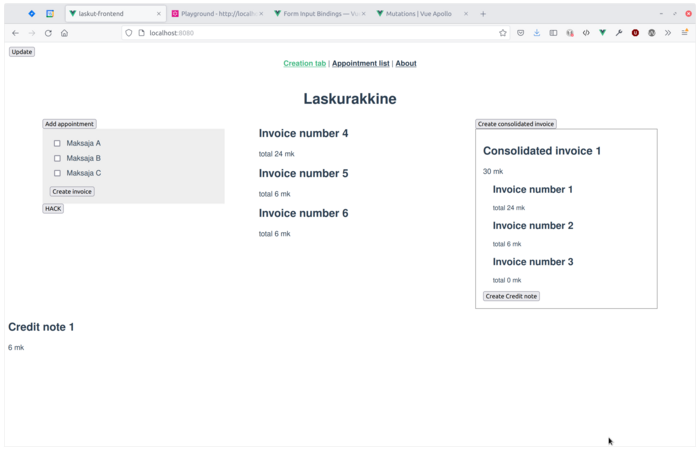
\includegraphics[width=\textwidth,height=0.6\textheight]{illustration/screenshots/Laskurakkine.png}
\caption{\label{rakkine_default-view}Laskujen lisäysnäkymä}
\end{figure}

Erillisessä listanäkymässä (Kuva \ref{rakkine_list-view}) voi
tarkastella luotujen käyntien tilaa sekä laskutettavan myynnin tilaa.
Ohjelma näyttää, onko käynti laskutettu vai laskuttamaton. Myynnin
osalta ohjelma näyttää, miten myynti jakautuu eri maksajille, ja onko
summa avoin, laskutettu vai hyvitetty.

\begin{figure}
\centering
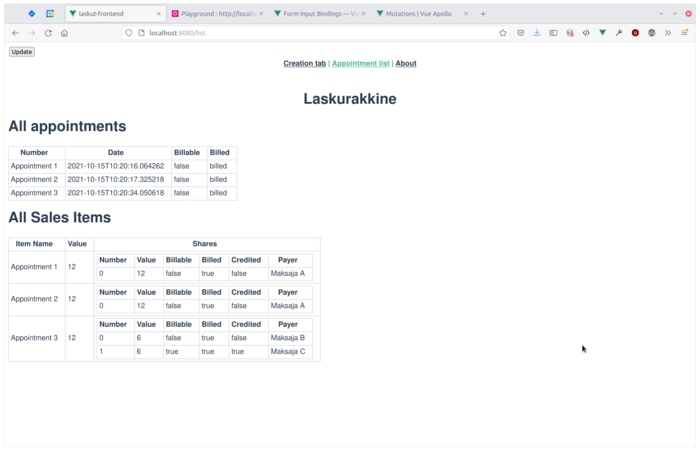
\includegraphics[width=\textwidth,height=0.6\textheight]{illustration/screenshots/List-view.png}
\caption{\label{rakkine_list-view}Ohjelman listanäkymä}
\end{figure}

\begin{figure}
\centering
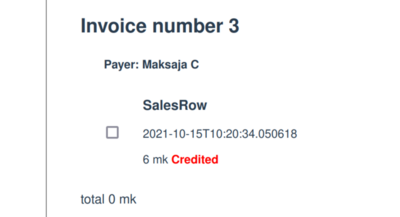
\includegraphics[width=\textwidth,height=0.6\textheight]{illustration/screenshots/credited.png}
\caption{\label{rakkine_credited}Ohjelma näyttää, että yksittäinen
laskurivi on hyvitetty}
\end{figure}

Kuvassa \ref{rakkine_credited} on esitetty miten ohjelma näyttää
hyvitetyn laskurivin.

\begin{figure}
\centering
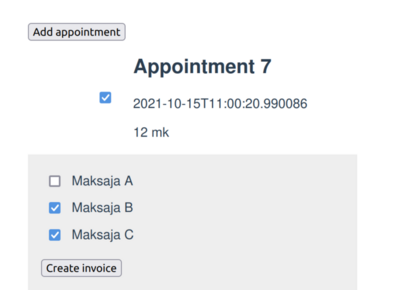
\includegraphics[width=\textwidth,height=0.6\textheight]{illustration/screenshots/Dividing.png}
\caption{\label{rakkine_dividing}Esimerkki käynnin jakamiesta usealle
maksajalle}
\end{figure}

Käytin asiakasohjelman tekemiseen niin vähän aikaa kuin mahdollista. Se
näkyy tyylin hiomattomuutena. Luonnosmaisen näköinen ulkoasu myös
kommunikoi muille prosessiin osallistuville, että ohjelmisto tai
etenkään sen käyttöliittymä ei ole tarkoitettu tuotantokäyttöön, vaan
apuvälineeksi erilaisten tietomallin piirteiden kartoittamiseen.

\hypertarget{kuvaus-tyuxf6mallista}{%
\section{Kuvaus työmallista}\label{kuvaus-tyuxf6mallista}}

Seuraavaksi kuvaan lyhyesti ne periaatteet, joiden varaan tämä työmalli
rakentuu.

\hypertarget{lyhyet-iteraatiot}{%
\subsection{Lyhyet iteraatiot}\label{lyhyet-iteraatiot}}

Lyhyet iteraatiot, joiden välissä pidetään suunnittelutapaaminen, ovat
ehdoton edellytys mallin ripeälle kehittämiselle. On tärkeää, että
iteraation kuluessa syntyy käyttökelpoinen ohjelmistoversio, jonka
avulla mallin toimivuutta voidaan testata ja todentaa.

\hypertarget{keskusteleva-suhde-tuoteomistajan-ja-kehittuxe4juxe4n-vuxe4lilluxe4}{%
\subsection{Keskusteleva suhde tuoteomistajan ja kehittäjän
välillä}\label{keskusteleva-suhde-tuoteomistajan-ja-kehittuxe4juxe4n-vuxe4lilluxe4}}

Koska tavoitteena on luoda kieli, jota voivat käyttää niin ohjelmoijat
kuin liiketoimintaväkikin, sen kehittämiseen luontevin ja
todennäköisesti ainoa tapa on rakentaa mallia keskustelevalla otteella.

\hypertarget{kuxe4yttuxe4juxe4tarinoihin-pohjautuva-tyuxf6lista}{%
\subsection{Käyttäjätarinoihin pohjautuva
työlista}\label{kuxe4yttuxe4juxe4tarinoihin-pohjautuva-tyuxf6lista}}

Ketterän kehityksen työkalupakista peräisin oleva ajatus
yksinkertaisista käyttäjätarinoista soveltuu hyvin tietomallin
kehittämisen lähtökohdaksi. Kun huomion keskipisteenä ovat ne asiat,
joita käyttäjä voi ohjelmistolla tehdä, on myös syntyvä malli lähempänä
alan realismia.

\hypertarget{rajapintaskeeman-rakentaminen-kuxe4sitteiden-pohjalta}{%
\subsection{Rajapintaskeeman rakentaminen käsitteiden
pohjalta}\label{rajapintaskeeman-rakentaminen-kuxe4sitteiden-pohjalta}}

GraphQL-rajapintaskeema kannattaa rakentaa ennenkuin kirjoittaa skeeman
toteuttavaa koodia. Näin kielen käsitteet ja niiden väliset suhteet
tulevat formaalisti ilmaistuksi. Ohjelmakoodin kirjoittamisen aikana
skeema saattaa myös tarkentua, ja silloin kannattaa muutokset tehdä
välittömästi.

\hypertarget{koodin-ja-mallin-pituxe4minen-luxe4hekkuxe4in}{%
\subsection{Koodin ja mallin pitäminen
lähekkäin}\label{koodin-ja-mallin-pituxe4minen-luxe4hekkuxe4in}}

Välttämätön osa tätä työtyyliä on koodin ja mallin vastaavuus. Mallissa
käytettävät käsitteet on löydyttävä koodista, ja koodissa tulisi olla
lähinnä vain nämä käsitteet ja niiden väliset suhteet sellaisina, kuin
ne \glslink{ubilang}{kaikenkattavassa kielessä} ilmenevät.

\hypertarget{voimakkaat-refaktoroinnit}{%
\subsection{Voimakkaat refaktoroinnit}\label{voimakkaat-refaktoroinnit}}

Voimakkaat refaktoroinnit ovat keino muokata koodin esittämästä mallista
joustava ja ilmaisuvoimainen. Nämä refaktoroinnit vaativat ehdottomasti
tuekseen jämerän yksikkötestisetin. Sen rakentaminen onnistuu
käytännössä vain testit edellä tekemällä.

\hypertarget{ohjelmoinnissa-vastaan-tulleet-ongelmat-jatkosuunnittelun-luxe4htuxf6kohtina}{%
\subsection{Ohjelmoinnissa vastaan tulleet ongelmat jatkosuunnittelun
lähtökohtina}\label{ohjelmoinnissa-vastaan-tulleet-ongelmat-jatkosuunnittelun-luxe4htuxf6kohtina}}

Suunnittelutapaamisten ja ohjelmointiprosessin välinen yhteys ei saa
olla vain yksisuuntainen. Mikäli suunnittelutapaaminen nähdään ainoana
osana prosessia, jossa suunnittelua tapahtuu ja ohjelmointi pelkästään
suunnitelmien mekaanisena toteuttamisena, hyödyt tästä
työskentelytyylistä jäävät hyvin vähäisiksi. Ohjelmointiprosessi on
suunnittelutyön toisenlainen vaihe, ja siinä ilmenevät ongelmat ovat
oivallinen maaperä seuraavan suunnittelutapaamisen aiheiksi.

\hypertarget{tyuxf6mallin-haasteita}{%
\section{Työmallin haasteita}\label{tyuxf6mallin-haasteita}}

Tämä työmalli vaatii ohjelmoijalta paljon. Se edellyttää jatkuvaa
kiinnostusta sovellusalueen piirteistä, ja laajaa tarkkaavuutta
suunnittelutapaamisten keskuisteluissa. Lisäksi se edellyttää kykyä
sietää epävarmuutta ja muuttaa suunnitelmia usein ja isosti. Teknisellä
tasolla työmalli edellyttää kykyä joustavan ohjelmiston
suunnittelemiseen, laajojen refaktorointien tekemiseen kireässä
aikataulussa pysyen ja tiukkaa keskittymistä niihin päämääriin, jotka
mallin kehittämisessä on kulloinkin asetettu.

Jotta tällainen työmalli voi olla hedelmällinen tuotantotasoisen
ohjelmiston tekemisessä, se edellyttää myös, että työtyyli ohjelmoijan
ympärillä vastaa tällaista tekemisen tapaa. Liiketoimintavetoisella
suunnittelulla on vaikutuksia paitsi ohjelmistotuotannon prosessiin,
myös sitä ympäröiviin prosesseihin, kuten asiakastarpeiden kokoamiseen
ja tulevan kehitystyön suunnittelemiseen.

\hypertarget{parannuksia-tietomalliin}{%
\section{Parannuksia tietomalliin}\label{parannuksia-tietomalliin}}

Viiden viikon aikana syntyi pieni malli laskutukseen tietorakenteen
parantamiseksi. Lisäksi löytyi kaksi pientä ideaa, joita voi hyödyntää,
kun ohjelmistoa kehitetään.

Pieni malli laskutuksen parantamiseksi on esitetty kuvassa
\ref{finalmodel1-again}. Se pitää sisällään ajatuksen käynnin
muuttumisesta myynniksi, kun se saapuu laskutuksen piiriin. Oma
erikoisuutensa on myös käynnin jakamiseen liittyvä jakoperuste - tätä ei
ohjelmistoon toteutettu, mutta suunnitteluvaiheessa se tuntui
hyödylliseltä idealta.

\begin{figure}
\centering
\includegraphics[width=\textwidth,height=0.3\textheight]{illustration/malli4.jpg}
\caption{\label{finalmodel1-again}Lopullinen malli}
\end{figure}

Kaksi pientä ideaa ovat molemmat käyttökelpoisia erillään mallista.
Ensimmäinen niistä on myynnin, myyntirivin ja hyvitysrivin välinen
tiivis yhteysketju. Tämä idea (kuva \ref{finalidea1})mahdollistaa hyvin
yksinkertaisen ja joustavan myynnin laskutus- ja hyvityslogiikan.

\begin{figure}
\centering
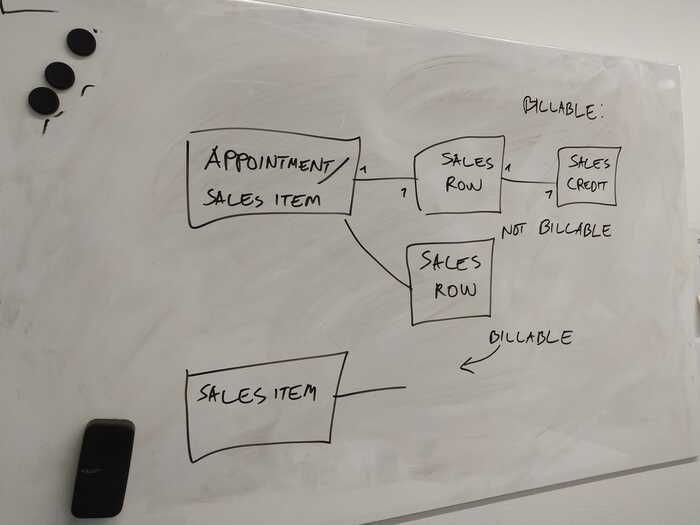
\includegraphics[width=\textwidth,height=0.3\textheight]{illustration/final-idea-1.jpg}
\caption{\label{finalidea1}Idea 1}
\end{figure}

Toinen pieni idea on, että käynti kannattaisi erottaa selkeästi laskulle
tulevasta myynnistä. Tällöin on mahdollista myös esimerkiksi vaihtaa
myöhemmin maksajaa, jolta käynti laskutetaan, ilman että jo
muodostettuihin laskuihin tarvitsee kajota. Tämä ajatus on esitetty
kuvassa \ref{finalidea2}.

\begin{figure}
\centering
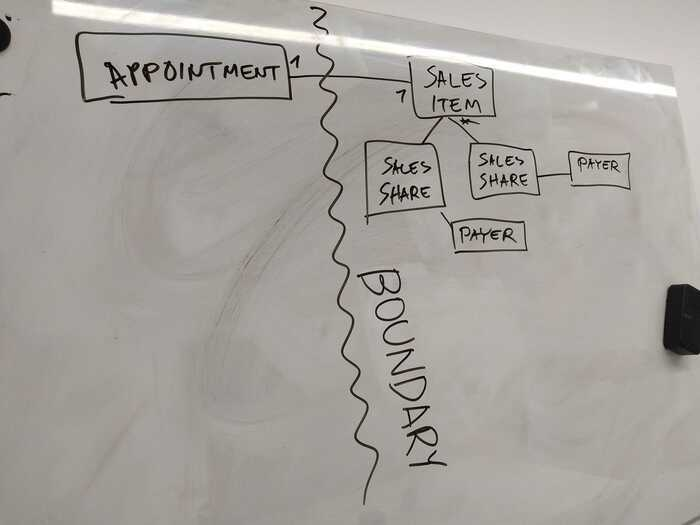
\includegraphics[width=\textwidth,height=0.3\textheight]{illustration/final-idea-2.jpg}
\caption{\label{finalidea2}Idea 2}
\end{figure}

\hypertarget{yhteenveto}{%
\chapter{Yhteenveto}\label{yhteenveto}}

Koodin kirjoittaminen on helppoa, mutta ihmisten ymmärtäminen vaikeaa.

Tähän pitäisi varmaan vielä arvioida omaa tekemistä.


% Sample content to demonstrate LaTeX command. You will likely delete this line and the
% next \input{sample/*} lines. You are also safe to delete the sample/ folder and its
% content once you refershed your LaTeX skills. Also check the appendix samples.
% \input{sample/1content.tex}
% \input{sample/2lorem.tex}
% \input{sample/3graph.tex}

%----------------------------------------------------------------------------------------
%	BIBLIOGRAPHY REFERENCES
%----------------------------------------------------------------------------------------

\input{style/biblio.tex}

%----------------------------------------------------------------------------------------
%	APPENDICES
%----------------------------------------------------------------------------------------

\input{style/appendix.tex}
%force smaller vertical spacing in table of content
%!!! There can be some fun depending if the appendices have (sub)sections or not :D
% You will have to play with these numbers and eventually add the \vspace line  before
% some \chapter and force another number.
% To add more fun, time to time the table of content get wrong after a build :(
\addtocontents{toc}{\vspace{11pt}}
\pretocmd{\chapter}{\addtocontents{toc}{\protect\vspace{-24pt}}}{}{}

\liite{1}% This is a hack to have right page numbering for each appendix. Make sure to
% use a unique number for each appendix.
\vspace{21.5pt}

\hypertarget{puxe4ivuxe4kirja-insinuxf6uxf6rityuxf6stuxe4}{%
\chapter{Päiväkirja
insinöörityöstä}\label{puxe4ivuxe4kirja-insinuxf6uxf6rityuxf6stuxe4}}

\hypertarget{viikko-1}{%
\section{Viikko 1}\label{viikko-1}}

Pidin palaverin Pasin ja Lauran kanssa. Sovimme taajaksi aihealueeksi
Diariumin laskutuksen. Varsinainen ongelma, johon keskitytään, on usean
maksajan laskut. Sanotaan, että hoitokäynnin lasku jaetaan kahtia,
asiakkaan maksamaan ja Kelan maksamaan osuuteen. Asiakkaan osuus
laskutetaan asiakkaalta, Kelan osuus taas Kelalta. Mutta Kela kieltäytyy
korvaamasta kyseistä käyntiä. Kirjanpidollisesti Kelalle lähetetty lasku
täytyy siis hyvittää. Mutta asiakkaalle lähetettyä laskua taas ei voi
hyvittää. Ja lisäksi täytyy voida ohjelmassa näyttää, että osa laskusta
on edelleen avoin.

Lauran kanssa yhdessä alettiin keskustella laskutuksesta. Laura näytti,
miten Diariumissa laskuttamisen logiikka toimii, ja piirsin
tussitaululle esimerkkejä, miten logiikka voisi toimia.

Käytin yksinkertaista notaatiota, jossa merkitsin asioita laatikoilla,
ja niiden välisiä yksi moneen -suhteita.

Piirsin aluksi käynnin. Niitä voi kuulua laskulle yksi tai useampia.
Laskut voidaan koostaa koontilaskuiksi. Koontilaskuja tai niiden osia
taas voidaan hyvittää luomalla hyvityslaskuja.

\begin{figure}
\centering
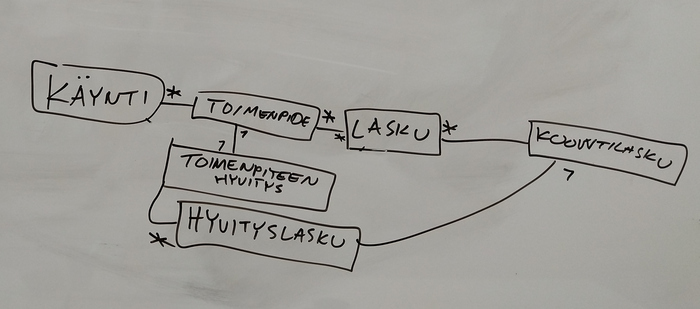
\includegraphics[width=\textwidth,height=0.3\textheight]{illustration/malli1.jpg}
\caption{\label{malli1}: Ensimmäinen malli}
\end{figure}

Oikeastaan käynnillä voi olla monta erillistä asiaa, ne ovat
laskutettavia toimenpiteitä. Palaverin lopuksi aikaansaatu kaavio on
kuvassa \ref{malli1}.

Tämä päätettiin toteuttaa.

Minulla meni torstaisen kokouksen jälkeen perjantai ja maanantai
perusrakenteen pystyttämiseen: Falcon, Ariadne GraphQL, Gunicorn ja
muutamia muita työkaluja. Lisäksi hommasin Pytest-testikirjaston, ja
opiskelin sen.

Lisäksi piti asentaa Apollo GraphQL-client ja Vue-cli, sekä plugin
Vue-Apollo.

Tiistaina sain ensimmäisen toiminnon, käyntien lisäämisen, valmiiksi.

Oli mielenkiintoista huomata, miten piirtämäni kuva ja tässä vaiheessa
aikaansaamani GraphQL-skeema muistuttivat läheisesti toisiaan.
GraphQL-queryjen sisältämät oliot rakensivat saman rakenteen, joka
tussitaululle piirsin. Sen sijaan GraphQL-mutaatioiden rooli ei ole
vielä auennut.

\hypertarget{viikko-2}{%
\section{Viikko 2}\label{viikko-2}}

Ensimmäisellä kehitykseen käyttämälläni viikolla (to-to) sain siis vain
ekan ominaisuuden valmiiksi. Sen jälkeen loppuviikosta tein vielä
käyntien laskutuksen. Lienee rehellistä arvioida, että noin viikon
kehitystyön myötä kaksi ``käyttäjätarinaa'' valmistui.

Perjantaina myös kirjoitin frontendia Vue-Apollolla ja käytin melkoisen
määrän aikaa kirjaston ominaisuuksien hahmottamiseen. Se ei kuulu
suoraan insinöörityön sisältöön, mutta toisaalta kuitenkin tarjoaa hyvän
kehyksen asioiden tekemiseen.

\hypertarget{viikko-3}{%
\section{Viikko 3}\label{viikko-3}}

Sain ensimmäisen version laskuhärvelistä valmiiksi. Tavoite oli Lauran
kanssa pitää asiasta palaveri perjantaina, mutta se peruuntui, koska
Laura oli tulossa kipeäksi.

Laskuhärveli toimii sinänsä, ja on hankala miettiä, onko siitä apua.

Kuitenkin domain-tason konseptien mallintaminen GraphQL-skeemaksi toimii
hyvin. Esimerkki, jossa koontilaskulla (ConsolidatedInvoice) voi olla
monta laskua (Invoice):

\begin{verbatim}
Type Invoice {
  number: Int
  sum: Float
  date: Date
}

type ConsolidatedInvoice {
  number: Int
  invoices: [Invoice]
}
\end{verbatim}

\hypertarget{palaveri-lauran-kanssa-tietomallin-kehittuxe4misestuxe4}{%
\section{27.9.2021 - Palaveri Lauran kanssa tietomallin
kehittämisestä}\label{palaveri-lauran-kanssa-tietomallin-kehittuxe4misestuxe4}}

Esittelin Lauralle tähän asti luomani softaproton. Pääasiallinen ongelma
on mielestäni laskun ja käynnin välisessä yhteydessä. Se, että laitetaan
käynti suoraan laskulle, on ongelmallista. Olin jo pitkin viikkoa
miettinyt, voisiko olla olemassa \textbf{Käyntirivi} ja \textbf{Käynnin
hyvitysrivi}, jotka sijaitsisivat laskulla ja koontilaskulla, ja
kumoaisivat toisensa.

Rupesin piirtämään Lauralle mallia, jossa Käynti liittyy Invoice-olioon,
ja Invoicea vastaa Credit Note, joka kumoaa Invoicella olevia käyntejä.
Piirsin Invoice- ja Credit note -olioiden sisään viivoja edustamaan
näitä käyntejä.

Laura totesi, että oikeastaan kirjanpidon kannalta täytyy täyttyä jokin
\textbf{Laskutusperuste}, jotta asia voidaan laskuttaa. Innostuin tästä
termistä, ja pyysin Lauraa jatkamaan. Laura sanoi, että laskutusperuste
on se, jonka pohjalta voidaan valita asioita laskutettavaksi. Asiat,
jotka täyttävät laskutusperusteen, mutta joihin ei liity laskua, voidaan
esimerkiksi listata laskuttamista varten. Pohjimmiltaan laskutusperuste
voi olla joko tavara tai palvelu, koska niitähän kaikki firmat myyvät.
Valitsimme laskutusperustetta kuvaamaan englanninkielisen termin
\textbf{BasisForInvoicing}. Palvelu on \textbf{Service}.

Ehdotin mallia, jossa \textbf{Appointment} voidaan viedä
\textbf{Invoicelle} \textbf{ServiceRow}-olioksi, jos täyttyy
BasisForInvoicing-ehto. Laura kurtisteli kulmiaan, eikä sanonut mitään.
Kysyin siis, eikö malli oikein miellytä, ja Laura totesi, että se
näyttää liian monimutkaiselta.

Pyyhin taulun puhtaaksi, ja kokeilimme uudestaan. Tein \textbf{Invoice}
-olion, jonka alle laitoin \textbf{ServiceRow} -nimisen olion. Invoicea
vastaamaan piirsin \textbf{CreditNote} -olion, jonka alle
\textbf{ServiceCreditRow}. Sivummas piirsin Appointment-olion, ja
pohdimme, mikä sen suhde voisi olla laskutukseen.

\begin{figure}
\centering
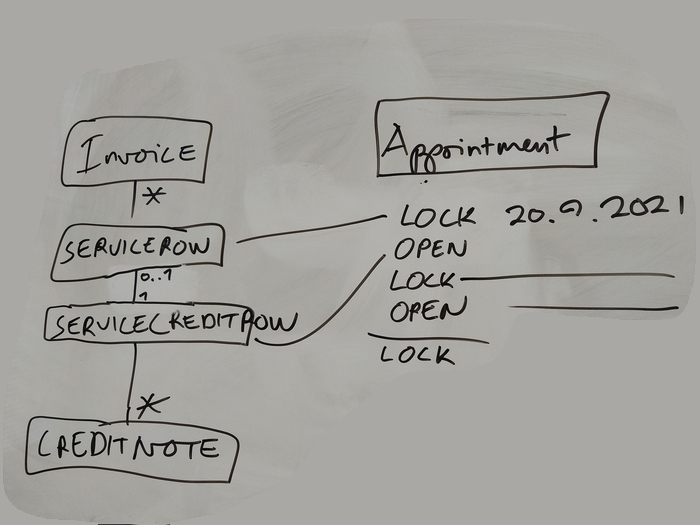
\includegraphics[width=\textwidth,height=0.5\textheight]{illustration/malli2.jpg}
\caption{\label{malli2}Toinen malli}
\end{figure}

Yhtäkkiä minulla välähti: mitä, jos tehtäisiin ikäänkuin loki
\textbf{Appointment}-olion sisälle: sinne tallennettaisiin
lukitustapahtuma, kun \textbf{Appointment} liitetään laskulle luomalla
sitä vastaava \textbf{ServiceRow}. Ja vastaavasti kun
\textbf{ServiceRow} hyvitettäisiin \textbf{ServiceCreditRown} avulla,
voitaisiin luoda avaustapahtuma. Näin ollen \textbf{Appointment}-luokan
alla olisi lista tapahtumia, ja listan avulla nähtäisiin sekä
laskutushistoria, että myös käynnin tämänhetkinen laskutustilanne:
Laskuttamatta vai avoinna? Esitän mallin kuvassa \ref{malli2}.

Laura huomautti, että tämä ei kuitenkaan ratkaise sitä pääongelmaa, joka
meillä on ollut: että käynnin hinta pitäisi jakaa monelle eri
maksajalle, joille lähetettyjä laskuja on voitava hyvittää itsenäisesti.

Niinpä pyyhin taas koko taulun puhtaaksi, ja lähdimme taas uudelleen
liikkeelle.

Nyt Käynnin alle lisättiin erillinen, laskutustarkoituksiin käytettävä
olio, jonka nimeksi pistettiin \textbf{BasisForInvoicing}. Tämä
BasisForInvoicing voidaan jakaa osiin, ja jokainen osa sisältää oman
erillisen listansa laskutustapahtumista: onko osa liitetty laskuun, vai
onko se hyvitetty ja taas siis avoinna.

\begin{figure}
\centering
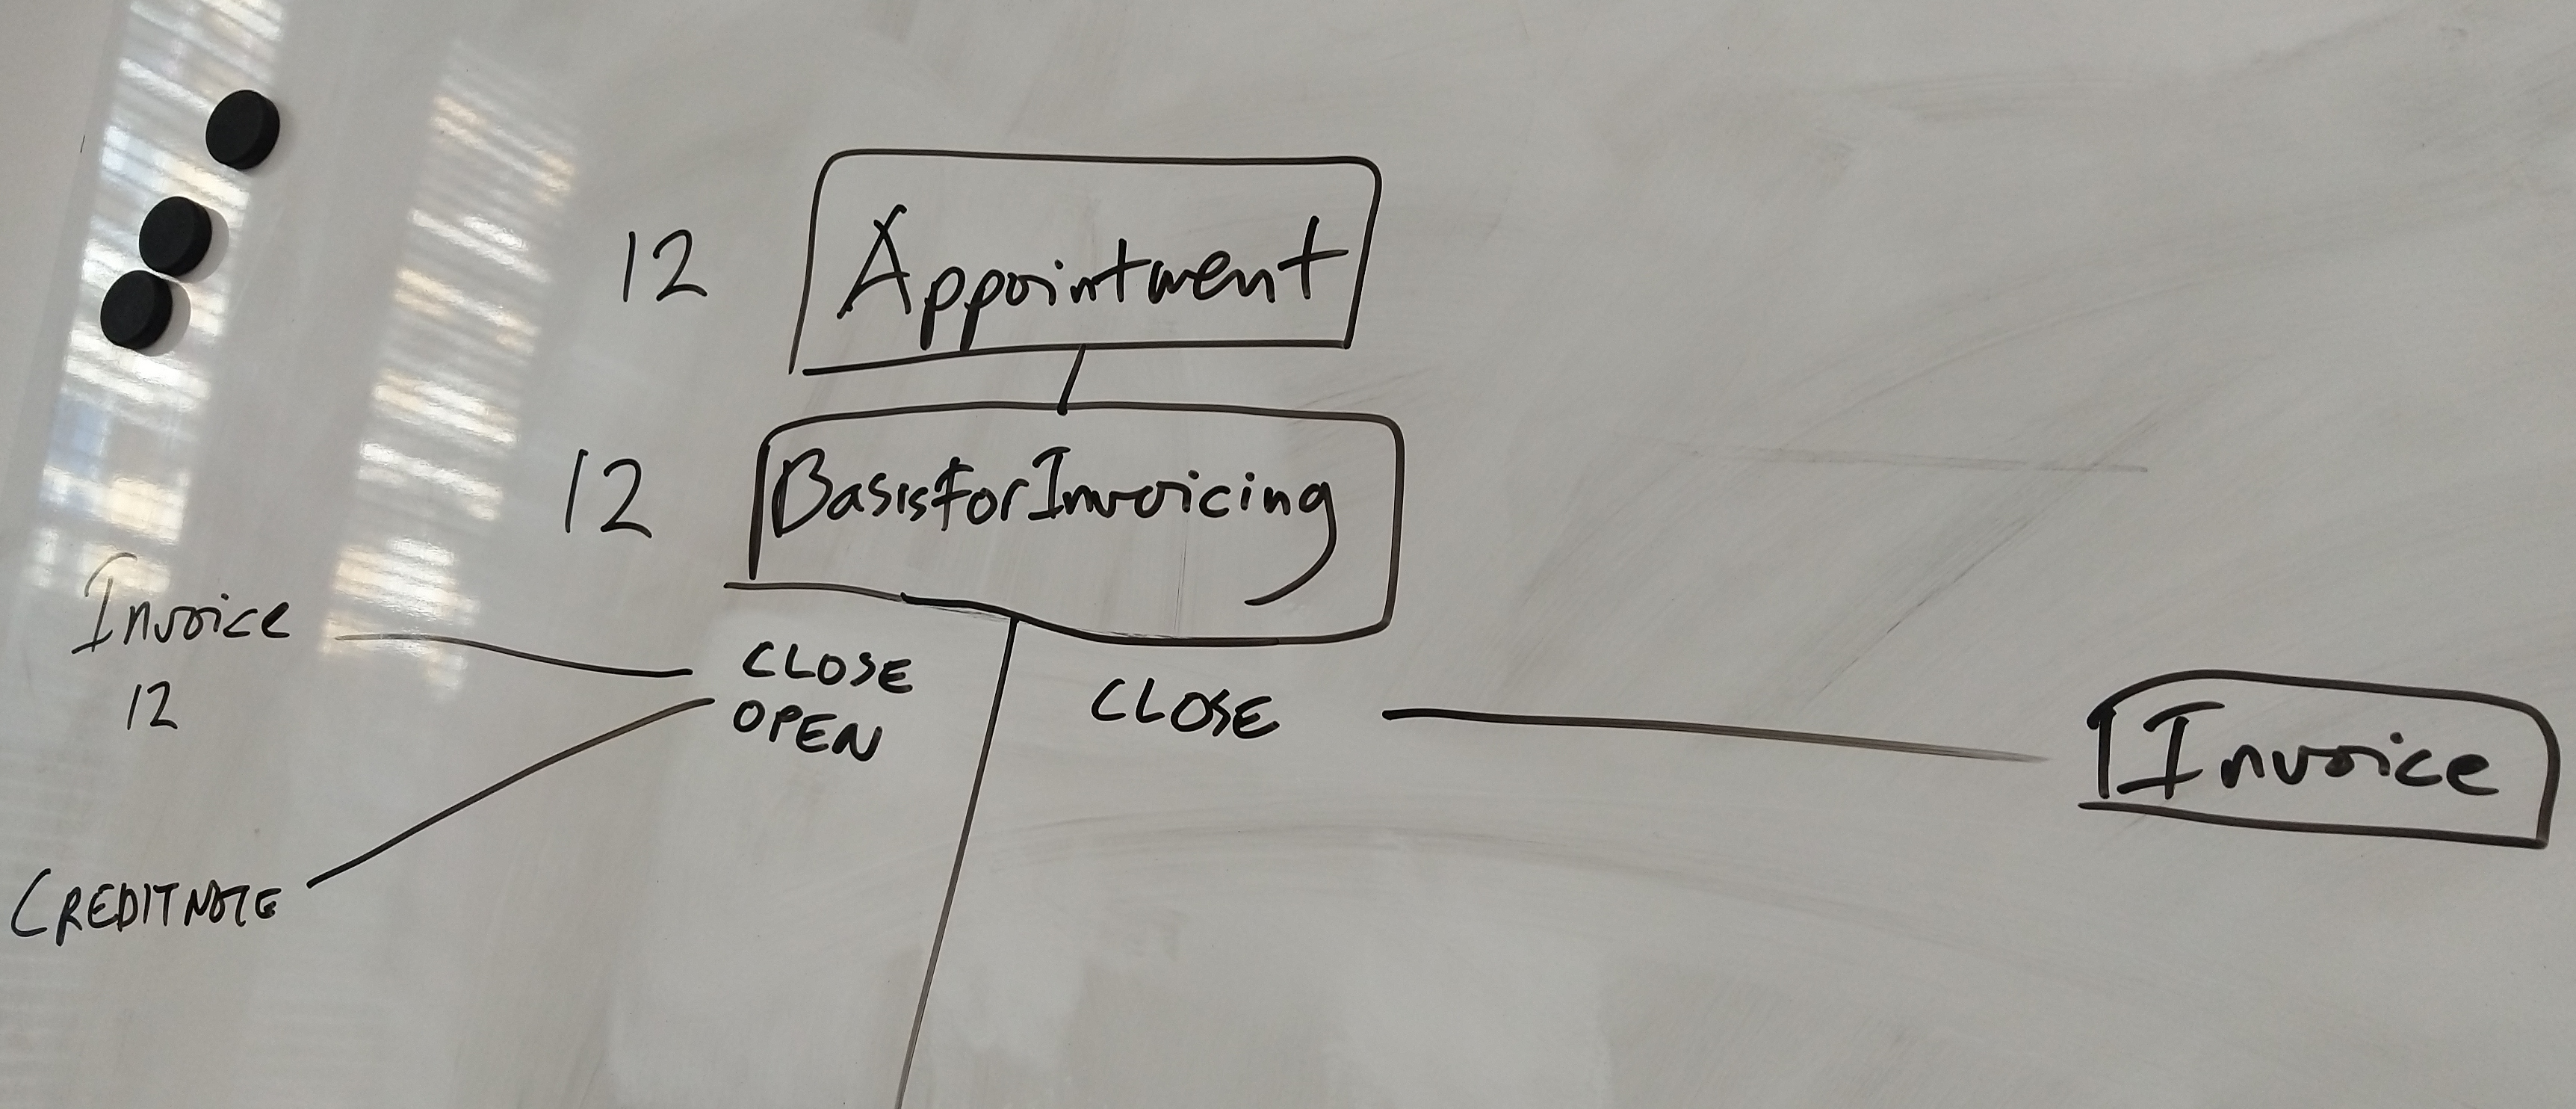
\includegraphics[width=\textwidth,height=0.5\textheight]{illustration/malli3.jpg}
\caption{\label{malli3}Kolmas malli}
\end{figure}

Tämä tuntui meistä hyvältä mallilta, ja sen pohjalta ryhdyin koodaamaan.
Tätä mallia esittää kuva \ref{malli3}. Sovittiin uusi palaveri viikon
päähän.
% Sample content to demonstrate appendix in LaTeX. You
% are safe to delete this lines (and the next samples) once you refreshed your LaTeX
% skills (and safe to delete the sample folder and all its file too).

%\addtocontents{toc}{\vspace{11pt}}%fix vertical space for Table of Content
% \liite{2}
% \input{sample/Xappendix2.tex}

% \addtocontents{toc}{\vspace{11pt}}
% \liite{3}
% \input{sample/X_R_example.tex}


%----------------------------------------------------------------------------------------
%	THIS IS THE END
%----------------------------------------------------------------------------------------
\end{document}
